\section{TP 11}
%\addcontentsline{toc}{section}{TP 11}

% \section*{Rappel}

% Structure du web:

% \begin{center}
% 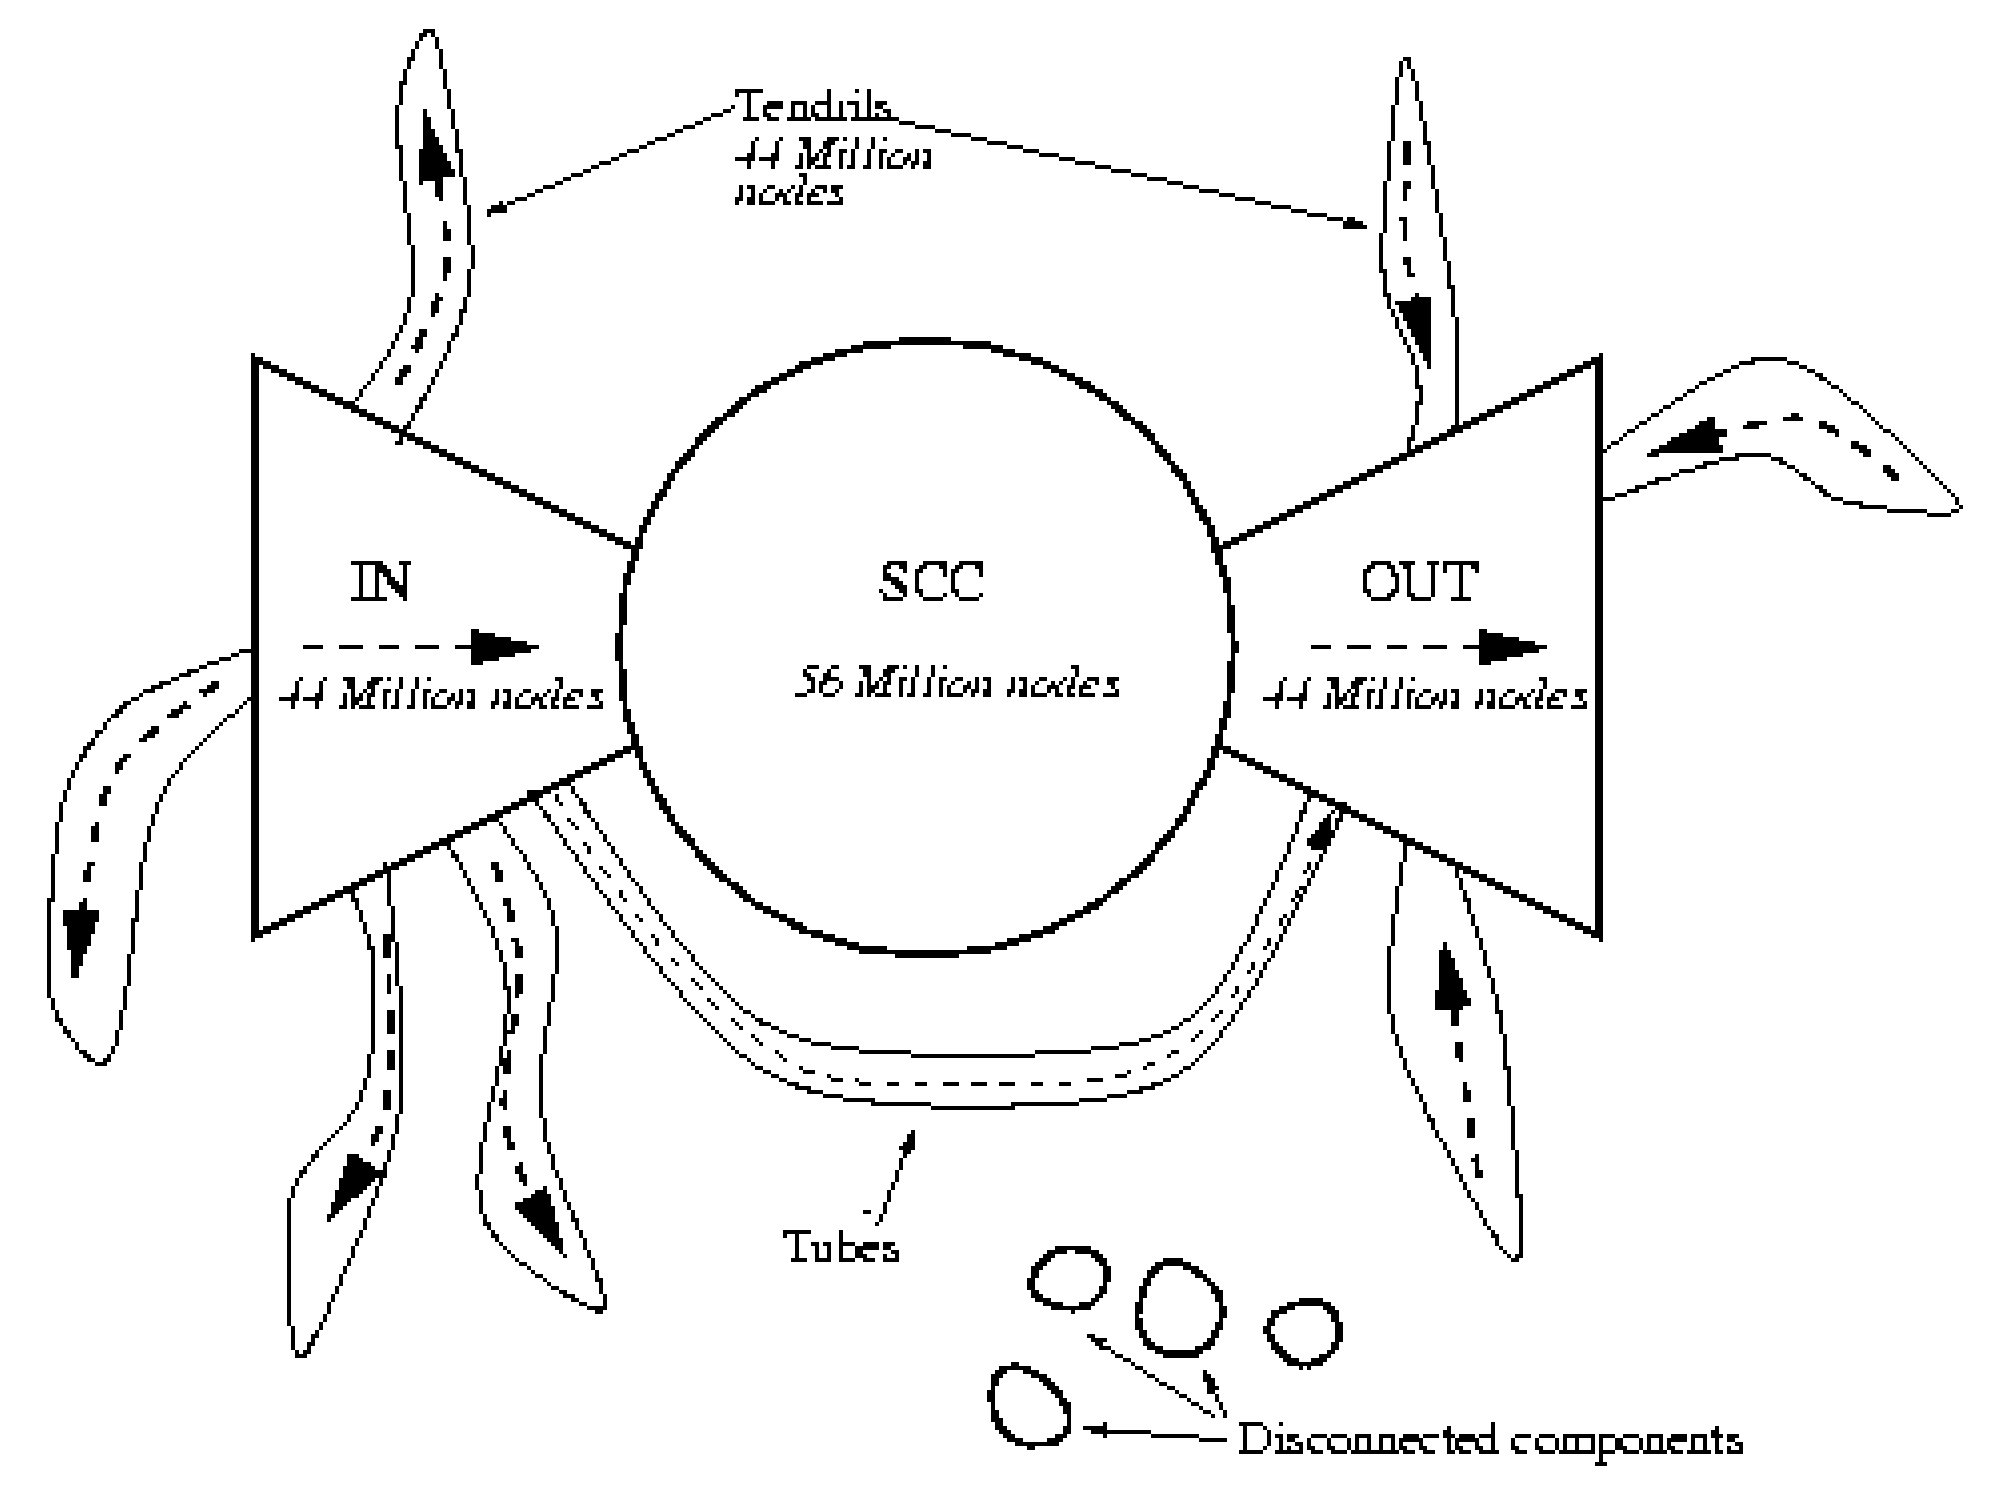
\includegraphics[scale = 0.5]{figs/web.png}
% \end{center}

% On repère trois composants principaux:
% \begin{itemize}
%  \item Un composant \textbf{in}, qui contient des liens hypertextes sortants.
%  \item Un composant fortement connecté principal, qui forme un \textbf{noyau} (SCC).
%  \item Un composant \textbf{out}, qui contient beaucoup de liens hypertextes entrants.
% \end{itemize}


% \newpage

% \section*{Exercices}


\subsection*{Exercice 1}
Considèrer de graphe avec 18 pages Web dans la Figure \ref{fig:webg}. Quels sont les noeuds qui font partie du noyau, les noeuds IN et les noeuds
OUT ? 

    \begin{figure}[h!]
    \begin{center}
    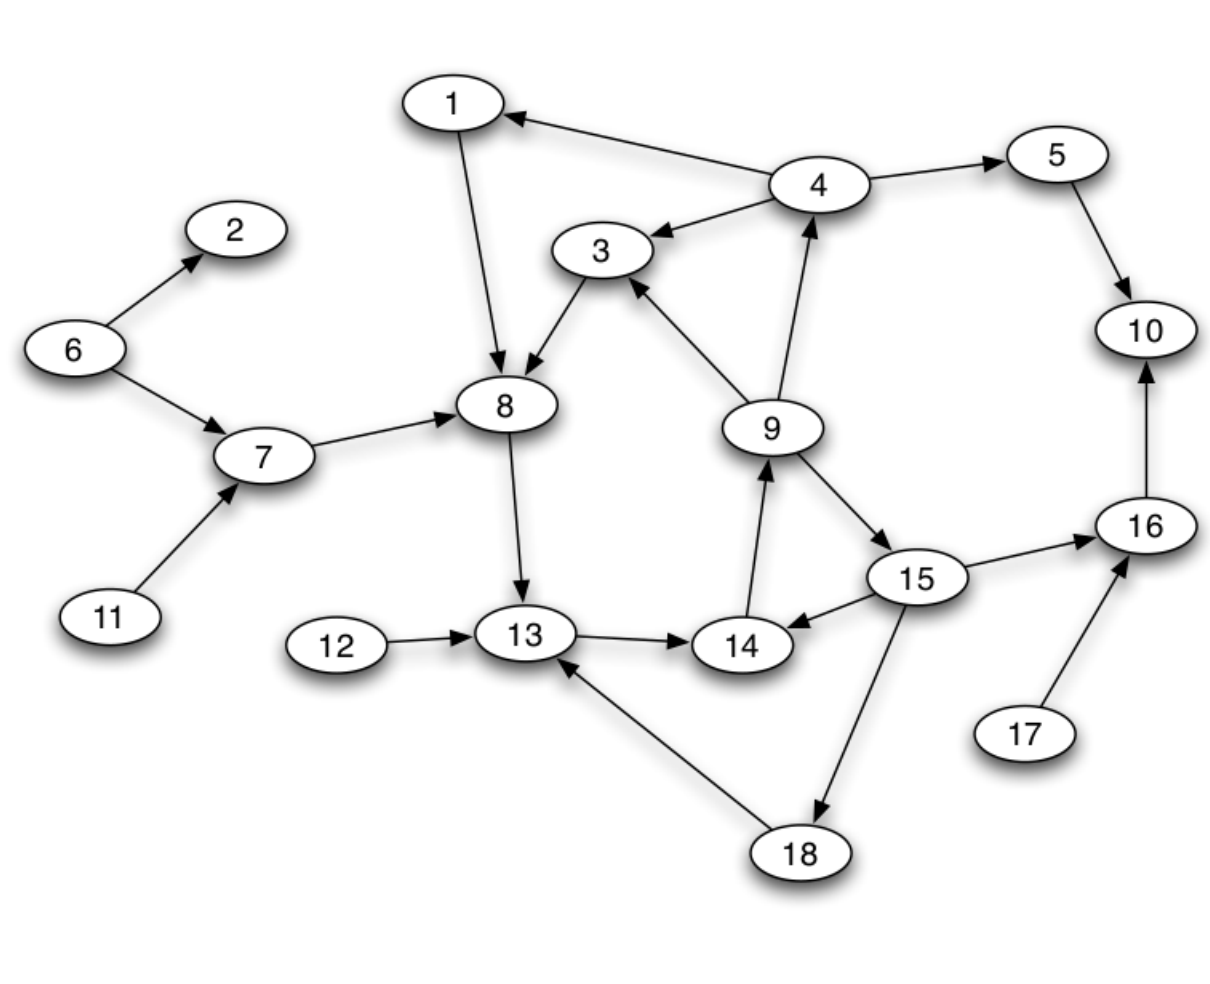
\includegraphics[scale = 0.3]{figs/graph.png}
    \end{center}
    \caption{Un graphe des pages web.}
    \label{fig:webg}
    \end{figure}

    \subsubsection*{Solution}

    \begin{center}
    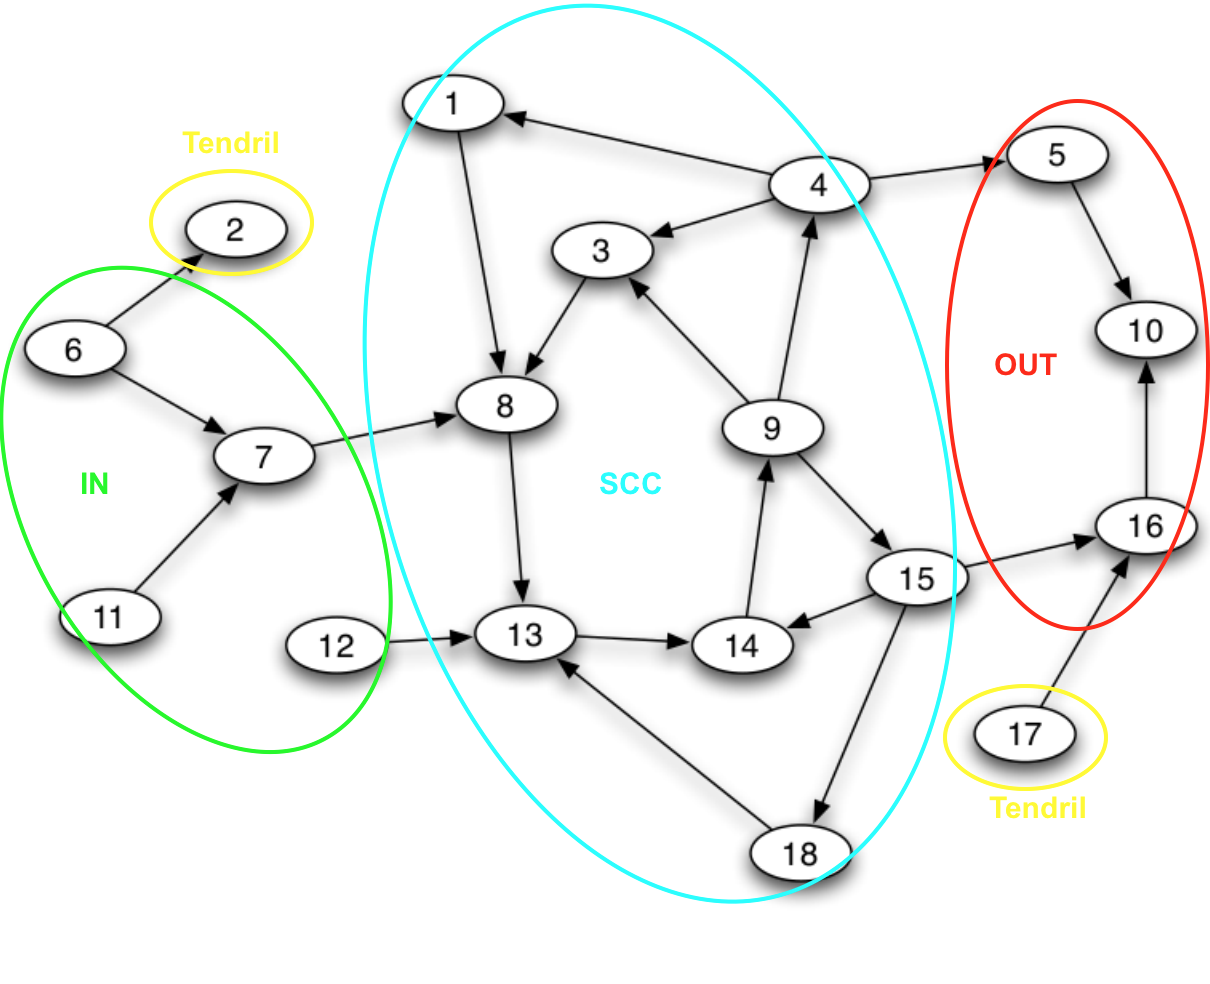
\includegraphics[scale=0.5]{figs/TP11Q1.png}
    \end{center}


\subsection*{Exercice 2}
Pour le graphe de la Figure \ref{fig:webg}.
\begin{enumerate}
 \item Montrez une arête tel que si on l'ajoute ou on la retire, on augmente la taille du noyau.
 \item Montrez une arête tel que si on l'ajoute ou on la retire, on augmente la taille de IN.
 \item Montrez une arête tel que si on l'ajoute ou on la retire, on augmente la taille de OUT.
\end{enumerate}

    \subsubsection*{Solution}

    \begin{center}
    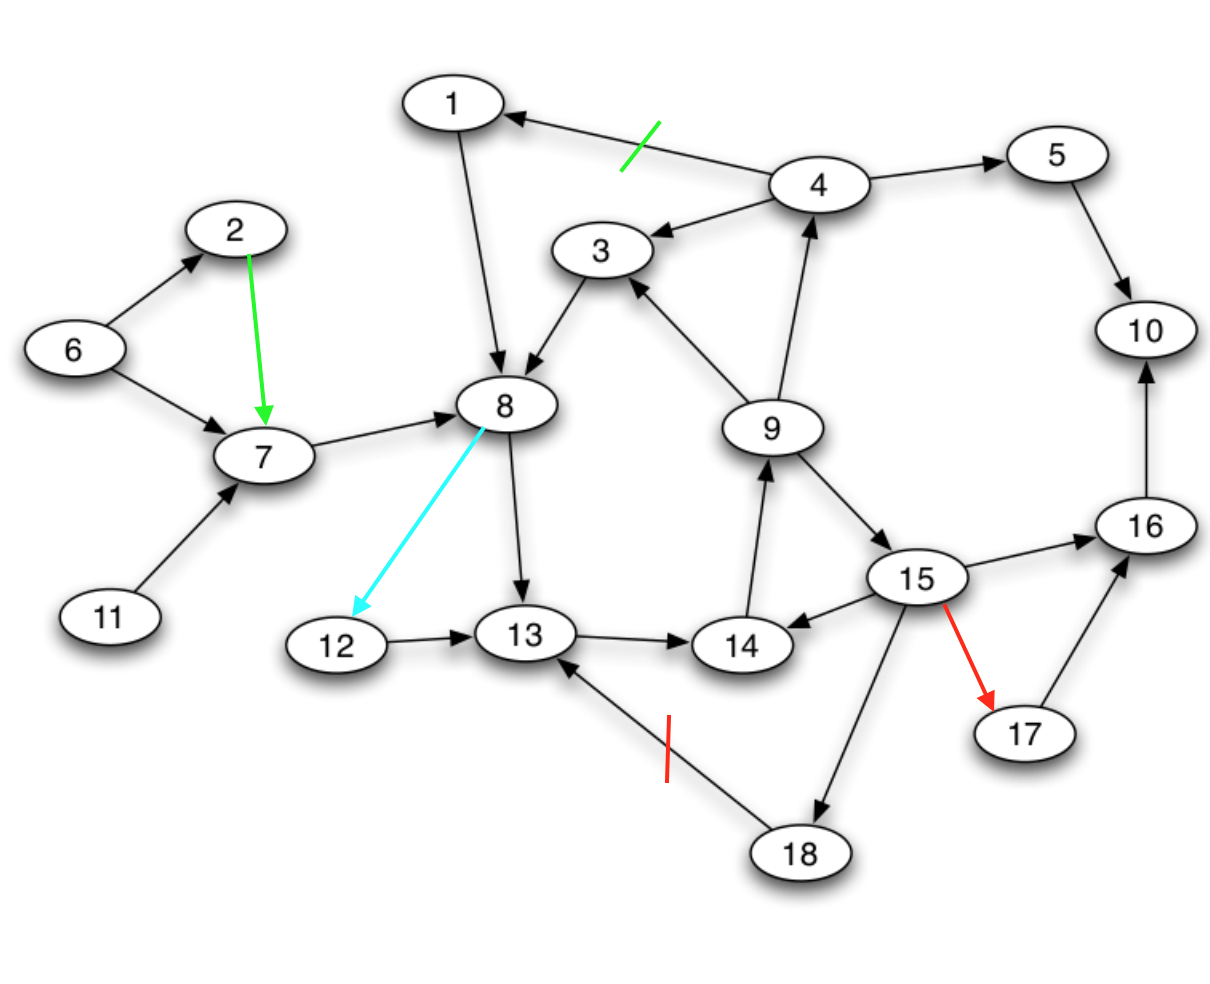
\includegraphics[scale=0.5]{figs/TP11Q2.png}
    \end{center}
    
    \begin{itemize}
        \item Le vert indique une arête à rajouter/retirer pour augmenter la taille du IN.
        \item Le rouge indique une arête à rajouter/retirer pour augmenter la taille du OUT.
        \item Le bleu indique une arête à rajouter pour augmenter la taille du SCC. Il n'est pas possible d'augmenter la taille du SCC en retirant une arête.
    \end{itemize}
    Il y a bien sûr d'autres possibilités que celles-là.


\subsection*{Exercice 3}
Décrivez un graphe tel qu'il existe une arête dont le retrait diminue la taille du noyeau d'au moins 1000 noeuds.

    \subsubsection*{Solution}
    Il faut pour cela un noyau qui possède un ensemble de 1000 noeuds ou plus qui n'est pas relié au IN ni au OUT et qui est relié au reste du noyau par seulement 2 arêtes : une entrante et une sortante.
    Supprimer l'arête qui va de cet ensemble au reste revient à rajouter l'ensemble au IN, tandis que supprimer l'autre arête revient à l'ajouter au OUT.


\subsection*{Exercice 4}
Décrivez un graphe tel qu'il existe une arête dont l'ajout diminue la taille de OUT d'au moins 1000 noueds.

    \subsubsection*{Solution}
    Il faut que le OUT possède une chaîne de 1000 noeuds ou plus et dont au moins un des noeuds de départ est directement lié au noyau.
    Il suffit de rajouter une arête au dernier noeud de cette chaîne pour qu'elle fasse partie intégrante du noyau, et donc pour diminuer la taille de OUT.

\subsection*{Exercice 5}
	\begin{enumerate}
	\item Calculez les valeurs de concentrateurs et d'autorités pour les pages dans le graphe présenté à la Figure \ref{fig:auth} après deux itérations.
	\item Quelles sont les valeurs une fois que la normalisation a été effectuée.
\end{enumerate}

\begin{figure}[!h]
	\centering
	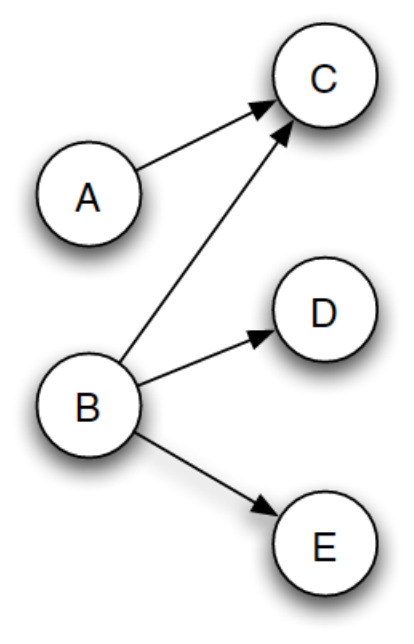
\includegraphics[scale=0.4]{figs/auth-hub.png}
	\caption{graphe de page web}
	\label{fig:auth}
\end{figure}

    \subsubsection*{Algorithme de normalisation}
    
    \begin{itemize}
        \item \textbf{Init} :  $ \forall x \: auth(x) = hub(x) = 1 $
        \item \textbf{Steps}: \\
            $\forall x \: auth(x) = \sum_{y \in hub(x)} hub(y)  $ \\
            $\forall x \: hub(x) = \sum_{y \in auth(x)} auth(y)  $
        \item \textbf{Normalisation} : \\
            $ \forall x \: auth(x) = \frac{auth(x)}{\sum auth} $ \\
            $ \forall x \: hub(x) = \frac{hub(x)}{\sum hub} $
    \end{itemize}

    \subsubsection*{Solution}
    \begin{itemize}
        \item \textbf{Auth} : authorité : liens entrants
        \item \textbf{Conc} : concentrateur : liens sortants
    \end{itemize}

    \begin{center}
    	\begin{tabular}{c|ccccc}
    	     & A & B & C & D & E\\ \hline
    	Auth & 1 & 1 & 1 & 1 & 1\\
    	Conc & 1 & 1 & 1 & 1 & 1\\ \hline
    	Auth & 0 & 0 & 2 & 1 & 1\\
    	Conc & 1 & 3 & 0 & 0 & 0\\ \hline
    	Auth & 0 & 0 & 4 & 3 & 3\\
    	Conc & 2 & 4 & 0 & 0 & 0\\ \hline
    	\end{tabular}
    \end{center}
    
    Normalisation :
    \begin{center}
    	\begin{tabular}{c|ccccc}
    	     & A & B & C & D & E\\ \hline
    	Auth & 0 & 0 & 0.4 & 0.3 & 0.3\\
    	Conc & $\frac{1}{3}$ & $\frac{2}{3}$ & 0 & 0 & 0\\ \hline
    	\end{tabular}
    \end{center}
    
    
\subsection*{Exercice 6}
Calculez les valeurs de PageRank pour chaque page dans le graphe présenté à la Figure \ref{fig:pagerank} après deux itérations avec S = 1.


\begin{figure}[ht!]
	\centering
	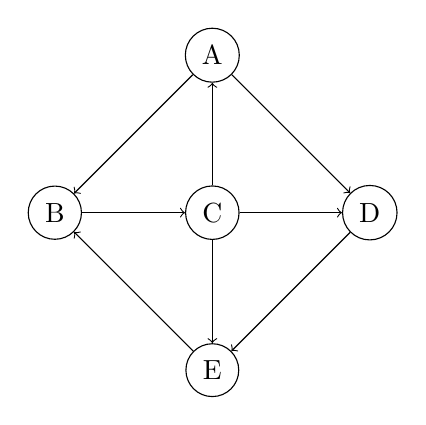
\begin{tikzpicture}[node distance=2cm]
		\tikzstyle{every node}=[draw=black,shape=circle]
		\node (c) at (0,0){C};
		\node[above of=c](a){A};
		\node[below of=c](e){E};
		\node[right of=c](d){D};
		\node[left of=c](b){B};

		\draw[->](a) -- (b);
		\draw[->](a) -- (d);
		\draw[->](b) -- (c);
		\draw[->](c) -- (a);
		\draw[->](c) -- (d);
		\draw[->](c) -- (e);
		\draw[->](d) -- (e);
		%\draw[->](d) -- (c);
		\draw[->](e) -- (b);
	\end{tikzpicture}
	\caption{graphe de page web}
	\label{fig:pagerank}
\end{figure}

    \subsubsection*{Solution}
    Règle de mise à jour : $Pr'(p) = S\ Pr(p) + (1-S) \frac{1}{n} = Pr(p)$.
    Seule la probabilité de suivre un lien à partir d'une page web entre en compte ici.\\
    À chaque itération k, on effectue les mises à jour suivantes :
    \begin{description}
        \item $Pr(A) = \frac{1}{3} Pr(C)$
        \item $Pr(B) = \frac{1}{2} Pr(A) + Pr(E)$
        \item $Pr(C) = Pr(B)$
        \item $Pr(D) = \frac{1}{2} Pr(A) + \frac{1}{3} Pr(C)$
        \item $Pr(E) = \frac{1}{3} Pr(C) + Pr(D)$
    \end{description}
    
    \begin{center}
        \begin{tabular}{c|ccccc}
        k & A & B & C & D & E\\ \hline 
    	0 & $\frac{1}{5}$ & $\frac{1}{5}$ & $\frac{1}{5}$ & $\frac{1}{5}$ & $\frac{1}{5}$\\ \\
    	1 & $\frac{1}{15}$ & $\frac{3}{10}$ & $\frac{1}{5}$ & $\frac{1}{6}$ & $\frac{4}{15}$\\ \\
    	2 & $\frac{1}{15}$ & $\frac{3}{10}$ & $\frac{3}{10}$ & $\frac{1}{10}$ & $\frac{7}{30}$\\
    	\end{tabular}
    \end{center}

\subsection*{Exercice 7}
Dans la Figure \ref{fig:equi}, les nombres à coté des noeuds représentent la valeur de PageRank de la page. Avec ce graphe, les valeurs de PageRank forment-elles un ensemble équilibré? Si oui pourquoi? Si non pourquoi?

\begin{figure}[ht!]
	\centering
	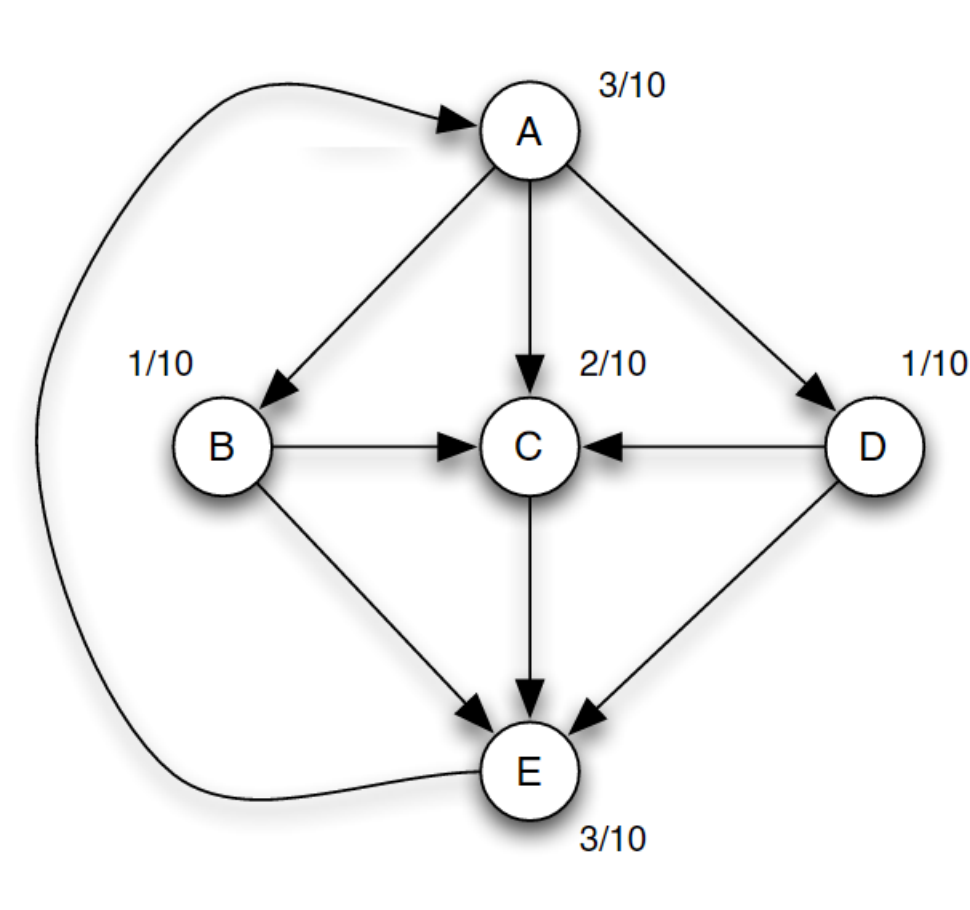
\includegraphics[scale=0.3]{figs/equi.png}
	\caption{graphe de page web}
	\label{fig:equi}
\end{figure}

    \subsubsection*{Solution}
    Il y a deux conditions à respecter pour que les valeurs de PageRank d'un graphe forment un ensemble équilibré :
    \begin{enumerate}
        \item La somme des valeurs doit valoir 1 : $\sum Pr(p_i) = 1$
        \item Une nouvelle itération doit donner les mêmes valeurs : $Pr'(p_i) = Pr(p_i) \ \forall p_i$\\
    \end{enumerate}
    
    Vérifions tout d'abord la première condition :
    $$ \sum Pr(p_i) = \frac{3}{10} + \frac{1}{10} + \frac{2}{10}  + \frac{1}{10}+  \frac{3}{10} = \frac{10}{10} = 1 $$

    Ensuite la seconde :
    \begin{description}
        \item $Pr'(A) = Pr(E) = \frac{3}{10} = Pr(A)$
        \item $Pr'(B) = \frac{1}{3} Pr(A) = \frac{1}{10} = Pr(B)$
        \item $Pr'(C) = \frac{1}{3} Pr(A) + \frac{1}{2} Pr(B) + \frac{1}{2} Pr(D) = \frac{2}{10} = Pr(C)$
        \item $Pr'(D) = \frac{1}{3} Pr(A) = \frac{1}{10} = Pr(D)$
        \item $Pr'(E) = \frac{1}{2} Pr(B) + Pr(C) + \frac{1}{2} Pr(D) = \frac{3}{10} = Pr(E)$\\
    \end{description}

    Nous pouvons donc conclure que nous cet ensemble de valeurs PageRank forme bien un ensemble équilibré.
    

\subsection*{Exercice 8}
		\begin{enumerate}
				\item Calculez les valeurs de PageRank pour chaque page dans le graphe présenté à la Figure \ref{fig:blackhole} après trois itérations avec S = 1.
				\item Que remarquez-vous? Selon vous comment vont évoluer les valeurs
						de PageRank pour un nombre d'itérations de plus en plus grand
				\item Calculez à nouveau les valeurs de PageRank pour chaque page mais pour 2 itérations avec S = 0.5.
		\end{enumerate}
		
    \begin{figure}[ht!]
	\centering
	
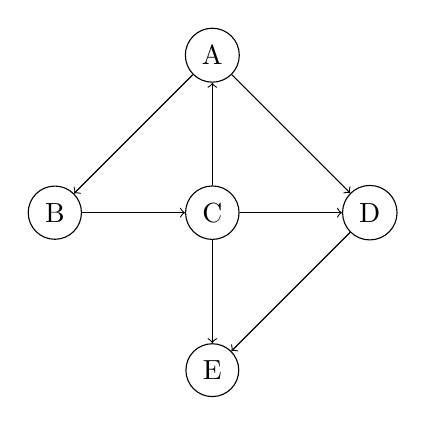
\begin{tikzpicture}[node distance=2cm]
	\tikzstyle{every node}=[draw=black,shape=circle]
	\node (c) at (0,0){C};
	\node[above of=c](a){A};
	\node[below of=c](e){E};
	\node[right of=c](d){D};
	\node[left of=c](b){B};

	\draw[->](a) -- (b);
	\draw[->](a) -- (d);
	\draw[->](b) -- (c);
	\draw[->](c) -- (a);
	\draw[->](c) -- (d);
	\draw[->](c) -- (e);
	\draw[->](d) -- (e);
	%\draw[->](d) -- (c);
	%\draw[->](e) -- (b);
\end{tikzpicture}
\caption{graphe de page web}
\label{fig:blackhole}
\end{figure}
		
    \subsubsection*{Solution}
    \begin{enumerate}
    
    \item Pour S=1, à chaque itération k, on effectue les mises à jour suivantes :
    \begin{description}
        \item $Pr(A) = \frac{1}{3} Pr(C)$
        \item $Pr(B) = \frac{1}{2} Pr(A)$
        \item $Pr(C) = Pr(B)$
        \item $Pr(D) = \frac{1}{2} Pr(A) + \frac{1}{3} Pr(C)$
        \item $Pr(E) = \frac{1}{3} Pr(C) + Pr(D) + Pr(E)$ \\
        \textit{(On ajoute $Pr(E)$ au calcul de E car c'est un noeud "cul-de-sac". Lors d'une itération, il faut prendre en compte le fait qu'une transition est bloquée au niveau de E et retombera donc vers E.)}
    \end{description}
    
    On obtient le résultat qui suit :
    \begin{center}
        \begin{tabular}{c|ccccc}
        k & A & B & C & D & E\\ \hline 
    	0 & $\frac{6}{30}$ & $\frac{6}{30}$ & $\frac{6}{30}$ & $\frac{6}{30}$ & $\frac{6}{30}$\\ \\
    	1 & $\frac{2}{30}$ & $\frac{3}{30}$ & $\frac{6}{30}$ & $\frac{5}{30}$ & $\frac{14}{30}$\\ \\
    	2 & $\frac{2}{30}$ & $\frac{1}{30}$ & $\frac{3}{30}$ & $\frac{3}{30}$ & $\frac{21}{30}$\\ \\
    	3 & $\frac{1}{30}$ & $\frac{1}{30}$ & $\frac{1}{30}$ & $\frac{2}{30}$ & $\frac{25}{30}$\\
    	\end{tabular}
    \end{center}
    
    \item On remarque qu'il y a une accumulation au niveau du noeud E.
    Sa valeur va tendre vers 1 alors que toutes les autres tendent vers 0.
    
    \item Pour S=0.5, à chaque itération k, on effectue les mises à jour suivantes :
    \begin{description}
        \item $Pr'(A) = \frac{1}{6} Pr(C) + \frac{1}{10}$
        \item $Pr'(B) = \frac{1}{4} Pr(A) + \frac{1}{10}$
        \item $Pr'(C) = \frac{1}{2} Pr(B) + \frac{1}{10}$
        \item $Pr'(D) = \frac{1}{4} Pr(A) + \frac{1}{6} Pr(C) + \frac{1}{10}$
        \item $Pr'(E) = \frac{1}{6} Pr(C) + \frac{1}{2} Pr(D) + \frac{1}{2} Pr(E) + \frac{1}{10}$
    \end{description}
    
    Le tableau résultant est :
    \begin{center}
        \begin{tabular}{c|ccccc}
        k & A & B & C & D & E\\ \hline 
    	0 & $\frac{6}{30}$ & $\frac{6}{30}$ & $\frac{6}{30}$ & $\frac{6}{30}$ & $\frac{6}{30}$\\ \\
    	1 & $\frac{4}{30}$ & $\frac{4.5}{30}$ & $\frac{6}{30}$ & $\frac{5.5}{30}$ & $\frac{10}{30}$\\ \\
    	2 & $\frac{4}{30}$ & $\frac{4}{30}$ & $\frac{5.25}{30}$ & $\frac{5}{30}$ & $\frac{11.75}{30}$\\
    	\end{tabular}
    \end{center}


\end{enumerate}